%%%%%%%%%%%%%%%%%%%%%%%%%%%%%%%%%%%%%%%%%%%%%%%%%%%%%%%%%%%%%%%%%%%%%%%%%%%%%%%%
%2345678901234567890123456789012345678901234567890123456789012345678901234567890
%        1         2         3         4         5         6         7         8

\documentclass[letterpaper, 10 pt, conference]{ieeeconf}  % Comment this line out
                                                          % if you need a4paper
%\documentclass[a4paper, 10pt, conference]{ieeeconf}      % Use this line for a4
                                                          % paper

\IEEEoverridecommandlockouts                              % This command is only
                                                          % needed if you want to
                                                          % use the \thanks command
\overrideIEEEmargins
% See the \addtolength command later in the file to balance the column lengths
% on the last page of the document

\usepackage[pdftex]{graphicx}
\graphicspath{{resources/}}

% The following packages can be found on http:\\www.ctan.org
%\usepackage{graphics} % for pdf, bitmapped graphics files
%\usepackage{epsfig} % for postscript graphics files
%\usepackage{mathptmx} % assumes new font selection scheme installed
%\usepackage{times} % assumes new font selection scheme installed
%\usepackage{amsmath} % assumes amsmath package installed
%\usepackage{amssymb}  % assumes amsmath package installed
\usepackage[T1]{fontenc}
\usepackage[utf8]{inputenc}
\usepackage{xspace}  

\newcommand{\diaspec}{Dia\-Spec\xspace}

\title{Using the \diaspec{} design language and compiler to develop
  robotics systems}

\author{%
  \parbox{3 in}{\centering Damien Cassou\\
    Software Architecture Group, HPI\\
    University of Potsdam, Germany\\%
    {\tt\small damien.cassou@hpi.uni-potsdam.de}}
  \hspace*{ 0.5 in}
  \parbox{3 in}{ \centering Serge Stinckwich and Pierrick Koch\\
    IRD, UMMISCO\\
    Hanoi, Vietnam\\
    {\tt\small serge.stinckwich@ird.fr}}
}

% \author{Damien Cassou and Serge Stinckwich and Pierrick Koch% <-this % stops a space
% %\thanks{This work was not supported by any organization}% <-this % stops a space
%   \thanks{H. Kwakernaak is with Faculty of Electrical Engineering,
%     Mathematics and Computer Science, University of Twente, 7500 AE
%     Enschede, The Netherlands {\tt\small h.kwakernaak@autsubmit.com}}%
%   \thanks{P. Misra is with the Department of Electrical Engineering,
%     Wright State University, Dayton, OH 45435, USA {\tt\small
%       pmisra@cs.wright.edu}}%
% }


\begin{document}

\maketitle
\thispagestyle{empty}
\pagestyle{empty}


%%%%%%%%%%%%%%%%%%%%%%%%%%%%%%%%%%%%%%%%%%%%%%%%%%%%%%%%%%%%%%%%%%%%%%%%%%%%%%%%
\begin{abstract}

These instructions provide basic guidelines for preparing camera-ready (CR)
Proceedings-style papers. This document is itself an example of the
desired layout for CR papers (inclusive of this abstract). The document
contains information regarding desktop publishing format, type sizes, and
type faces. Style rules are provided that explain how to handle equations,
units, figures, tables, references, abbreviations, and acronyms. Sections
are also devoted to the preparation of the references and acknowledgments.

\end{abstract}

%!TEX root=dslrob.tex
\section{Introduction}

A Sense/Compute/Control (SCC) application is one that interacts with
the environment~\cite{Tayl09a}. The SCC architectural pattern
guides the description of SCC applications and involves four kinds of
components, organized into layers~\cite{Cass11a,Edwar09a}: (1)
\emph{sensors} at the bottom, which obtain information about the
environment; (2) then \emph{context operators}, which process this
information; (3) then \emph{control operators}, which use this refined
information to control (4) \emph{actuators} at the top, which finally
impact the environment. A robotics application is a kind of SCC
application where the environment is composed of a robot
(sensors/actuators/body, control architecture, \etc{}) and the robot's
neighborhood (the walls, ground, people, \etc{})~\cite{Sicil08a}. As
noticed by Taylor \etal{}~\cite{Tayl09a}, the Sense/Plan/Act
architecture~\cite{Sicil08a}, widely used in robotics, closely
resembles the SCC architectural pattern.

\diaspec{} is a domain-specific design language dedicated to
describing SCC applications~\cite{Cass09b,Cass11a}. From such a design
description, the \diaspec{} compiler produces a dedicated Java
programming framework that is both \emph{prescriptive} and
\emph{restrictive}: it is prescriptive in the sense that it guides the
developer, and it is restrictive in the sense that it limits the
developer to what the design description allows. By separating
application logic (implemented by the developers) and runtime support
(generated in the programming framework), \diaspec{} facilitates the
design, implementation and evolution of SCC applications.

%\damien{Talk about problems in the robotics domain: ad-hoc solutions, hard to reuse, hard to adapt to new environments...}

\subsection*{Contributions}

Our contributions are as follows:

\begin{itemize}
\item \emph{A report} on an experiment of designing and implementing a
  standard robotics application in the SCC architectural pattern with
  the \diaspec{} domain-specific design language and framework
  (Sections~\ref{sec:designing} and~\ref{sec:implementing}). This
  report includes detailed instructions and guidelines to allow
  further experiments.
\item \emph{A discussion} of the benefits and problems of using
  \diaspec{} in a robotics setting (Section~\ref{sec:discussing}).
  This discussion includes a list of changes to \diaspec{} that would
  make it a better framework for developing new robotics applications.
\end{itemize}

We finally highlight some related works and conclude in
sections~\ref{sec:related} and~\ref{sec:conclusion}.

%%% LocalWords:  SCC




An SCC application can be defined according to an architectural
pattern involving four kinds of components, organized into layers: (1)
\emph{sensors} at the bottom, which obtain information about the
environment; (2) then \emph{context operators}, which process this
information; (3) then \emph{control operators}, which use this refined
information to control (4) \emph{actuators} at the top, which finally
impact the environment.

\begin{figure}
  \centering
  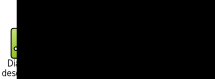
\includegraphics[width=\linewidth]{diaspec-process}
  \caption{Overview of the \diaspec{} development process}
  \label{fig:diaspec-process}
\end{figure}

\diaspec{} is a design language dedicated to describing SCC
applications. From such a design description, the \diaspec{} compiler
produces a dedicated Java programming framework
(Figure~\ref{fig:diaspec-process}) that is both \emph{prescriptive}
and \emph{restrictive}: it is prescriptive in the sense that it guides
the developer, and it is restrictive in the sense that it limits the
developer to what the design description allows. For each component
description in the design, the compiler generates an abstract class.
The abstract methods in this class represent code to be provided by
the developer, to allow him to program the application logic. To
implement a component, the developer implements these methods in a
subclass of this abstract class and thus never modifies generated
code.

By separating application logic (implemented by the developers) and
runtime support (generated in the programming framework), \diaspec{}
facilitates the design, implementation and evolution of SCC
applications. In the rest of this paper, we assume that robotics
applications are a subset of SCC applications and demonstrate that
\diaspec{} can be applied in the robotics domain.

%%% Local Variables:
%%% mode: latex
%%% coding: utf-8
%%% TeX-master: "dslrob"
%%% TeX-PDF-mode: t
%%% ispell-local-dictionary: "english"
%%% End:


\end{document}

%%% Local Variables: 
%%% mode: latex
%%% TeX-master: t
%%% TeX-PDF-mode: t
%%% coding: utf-8
%%% ispell-local-dictionary: "english"
%%% End:
